Задача оптимального транспорта (Optimal Transport)\cite{villani2009optimal} является одним из ключевых понятий 
в области теории вероятностей и машинного обучения.
Она представляет собой проблему определения оптимального способа перемещения вероятностной массы из одной распределенной системы
в другую с минимальными затратами или стоимостью. 
Основная идея заключается в том, чтобы найти наилучшее соответствие между двумя распределениями, учитывая их форму и объем.

\textit{Определение} \textbf{Оптимальный транспорт} (Монге) вводится путем рассмотрения двух вероятностных распределений \( \mu \) и \( \nu \) на двух метрических пространствах \( \mathcal{X} \) и \( \mathcal{Y} \). Задача состоит в поиске отображения \( T: \mathcal{X} \rightarrow \mathcal{Y} \), которое переводит распределение \( \mu \) в распределение \( \nu \), минимизируя некоторую функцию стоимости. Функция стоимости обычно является мерой сходства между элементами из \( \mathcal{X} \) и \( \mathcal{Y} \), такой как квадрат расстояния. Математически задача Монге формулируется как:
$$
    \inf_{\gamma \in \Pi(\mu, \nu)} \int_{\mathcal{X} \times \mathcal{Y}} c(x,y) \, d\gamma(x,y)
$$

,где \( \Pi(\mu, \nu) \) обозначает множество всех возможных совместных распределений 
\( \gamma \) на \( \mathcal{X} \times \mathcal{Y} \) с фиксированными маргинальными
распределениями \( \mu \) и \( \nu \), а \( c(x,y) \) — функция стоимости перевозки массы из \( x \) в \( y \).

\textit{Определение} \textbf{Оптимальный транспорт} (Кантарович) вводит понятие потенциала.
 Задача состоит в поиске потенциала \( \phi: \mathcal{X} \rightarrow \mathbb{R} \), который минимизирует функционал стоимости:

$$
    \inf_{\phi} \left( \int_{\mathcal{X}} \phi(x) \, d\mu(x) + \int_{\mathcal{Y}} \psi(y) \, d\nu(y) \right),
$$

где \( \psi \) — обратная функция к \( \phi \). Таким образом, отображение \( T: \mathcal{X} \rightarrow \mathcal{Y} \) получается из градиента потенциала.

Постановка Кантарович является релаксацией условий Монге .

\begin{figure}[h]
    \centering
    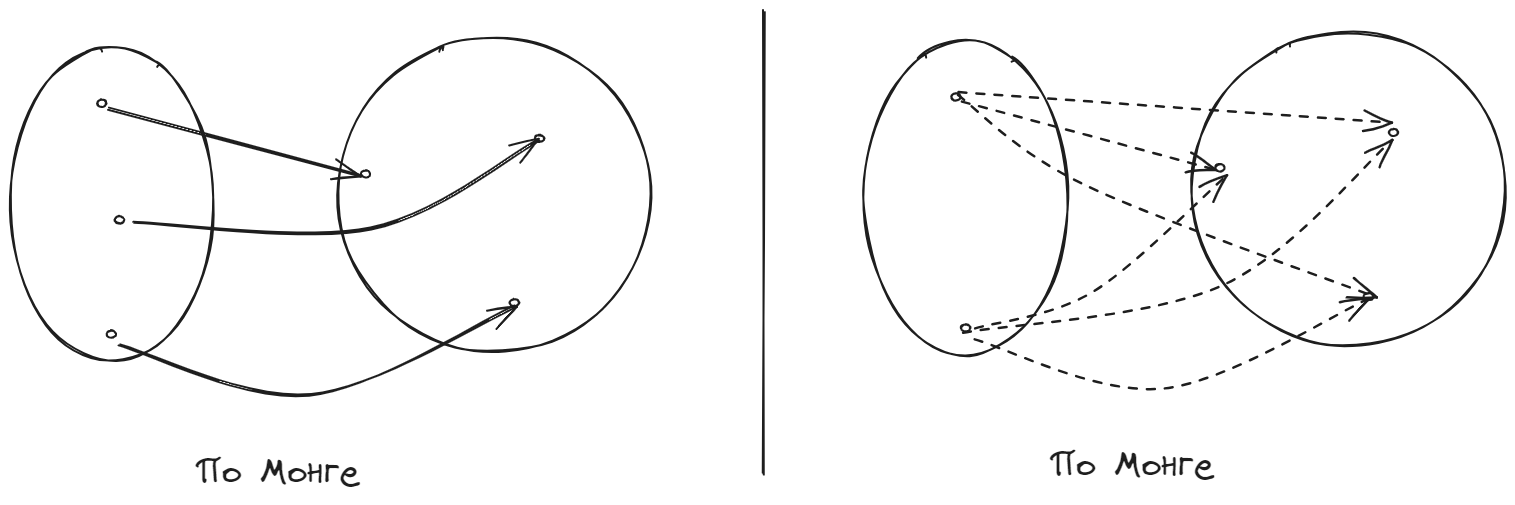
\includegraphics[width=0.5\textwidth]{assets/ml/generation/optimal_transport.excalidraw.png}
    \caption{Различие в подходе по Монге и Кантаровичу}
    \label{opt_transport}
\end{figure}
